%%%%%%%%%%%%%%%%%%%%%%%%%%%%%%%%%%%%%%%%%%%%%%%%%%%%%%%%%%%%%%%%%%%%%%%%%%%%%%%%
% Uncertainties and Results:
%%%%%%%%%%%%%%%%%%%%%%%%%%%%%%%%%%%%%%%%%%%%%%%%%%%%%%%%%%%%%%%%%%%%%%%%%%%%%%%%
\chapter{Statistical Analysis, Uncertainties and Results}
\label{statAnalysis_uncerts_results}
%%%%%%%%%%%%%%%%%%%%%%%%%%%%%%%%%%%%%%%%%%%%%%%%%%%%%%%%%%%%%%%%%%%%%%%%%%%%%%%%
The results and their uncertainties obtained in this search are presented here.  Evidence in 
support of a \WR and \nul signal was sought in finite sized windows of $\Mlljj$, whose sizes 
were chosen to minimize the upper bound \WR cross section limit in the absence of a signal.  
Uncertainties that affected the background and signal estimates were measured in each $\Mlljj$ 
window.  The main uncertainties that affected the background estimate arose from limited event 
statistics in $e\mu$ data, and discrepancies between data and simulations in \DY-rich control 
regions.  The main uncertainties that affected the signal estimate came from luminosity and 
pileup measurements in data.  Additional sources of uncertainty existed and were measured, 
but had a smaller cumulative impact on the results.  Following uncertainty estimation, the 
results were obtained by comparing data, expected SM backgrounds and hypothetical 
\WR and \nul signals using the $\Mlljj$ distribution, and limits on the \WR cross section, 
$\mWR$ and $\mnul$ masses derived from data and expected backgrounds.

%%%%%%%%%%%%%%%%%%%%%%%%%%%%%%%%%%%%%%%%%%%%%%%%%%%%%%%%%%%%%%%%%%%%%%%%%%%%%%%%
% Statistical Analysis 
%%%%%%%%%%%%%%%%%%%%%%%%%%%%%%%%%%%%%%%%%%%%%%%%%%%%%%%%%%%%%%%%%%%%%%%%%%%%%%%%
\section{Statistical Analysis}
\label{sec:massWindows}
%%%%%%%%%%%%%%%%%%%%%%%%%%%%%%%%%%%%%%%%%%%%%%%%%%%%%%%%%%%%%%%%%%%%%%%%%%%%%%%%
The \WR and \nul signals considered in this search were characterized by $\Mlljj$ distributions 
that peaked at \mWR, and had tails that extended several hundred $\GeV$ below and above the 
peak.  The only other assumption made regarding the shape of signals in $\Mlljj$ was that 
the tails grew larger as \mWR increased, as shown in Figure \ref{fig:fig:signalShapesAfterSelection}.  
This feature motivated the use of finite size $\Mlljj$ windows to search for evidence of LRS 
models.

\begin{figure}[btp]
	\centering
	\subfigure{
		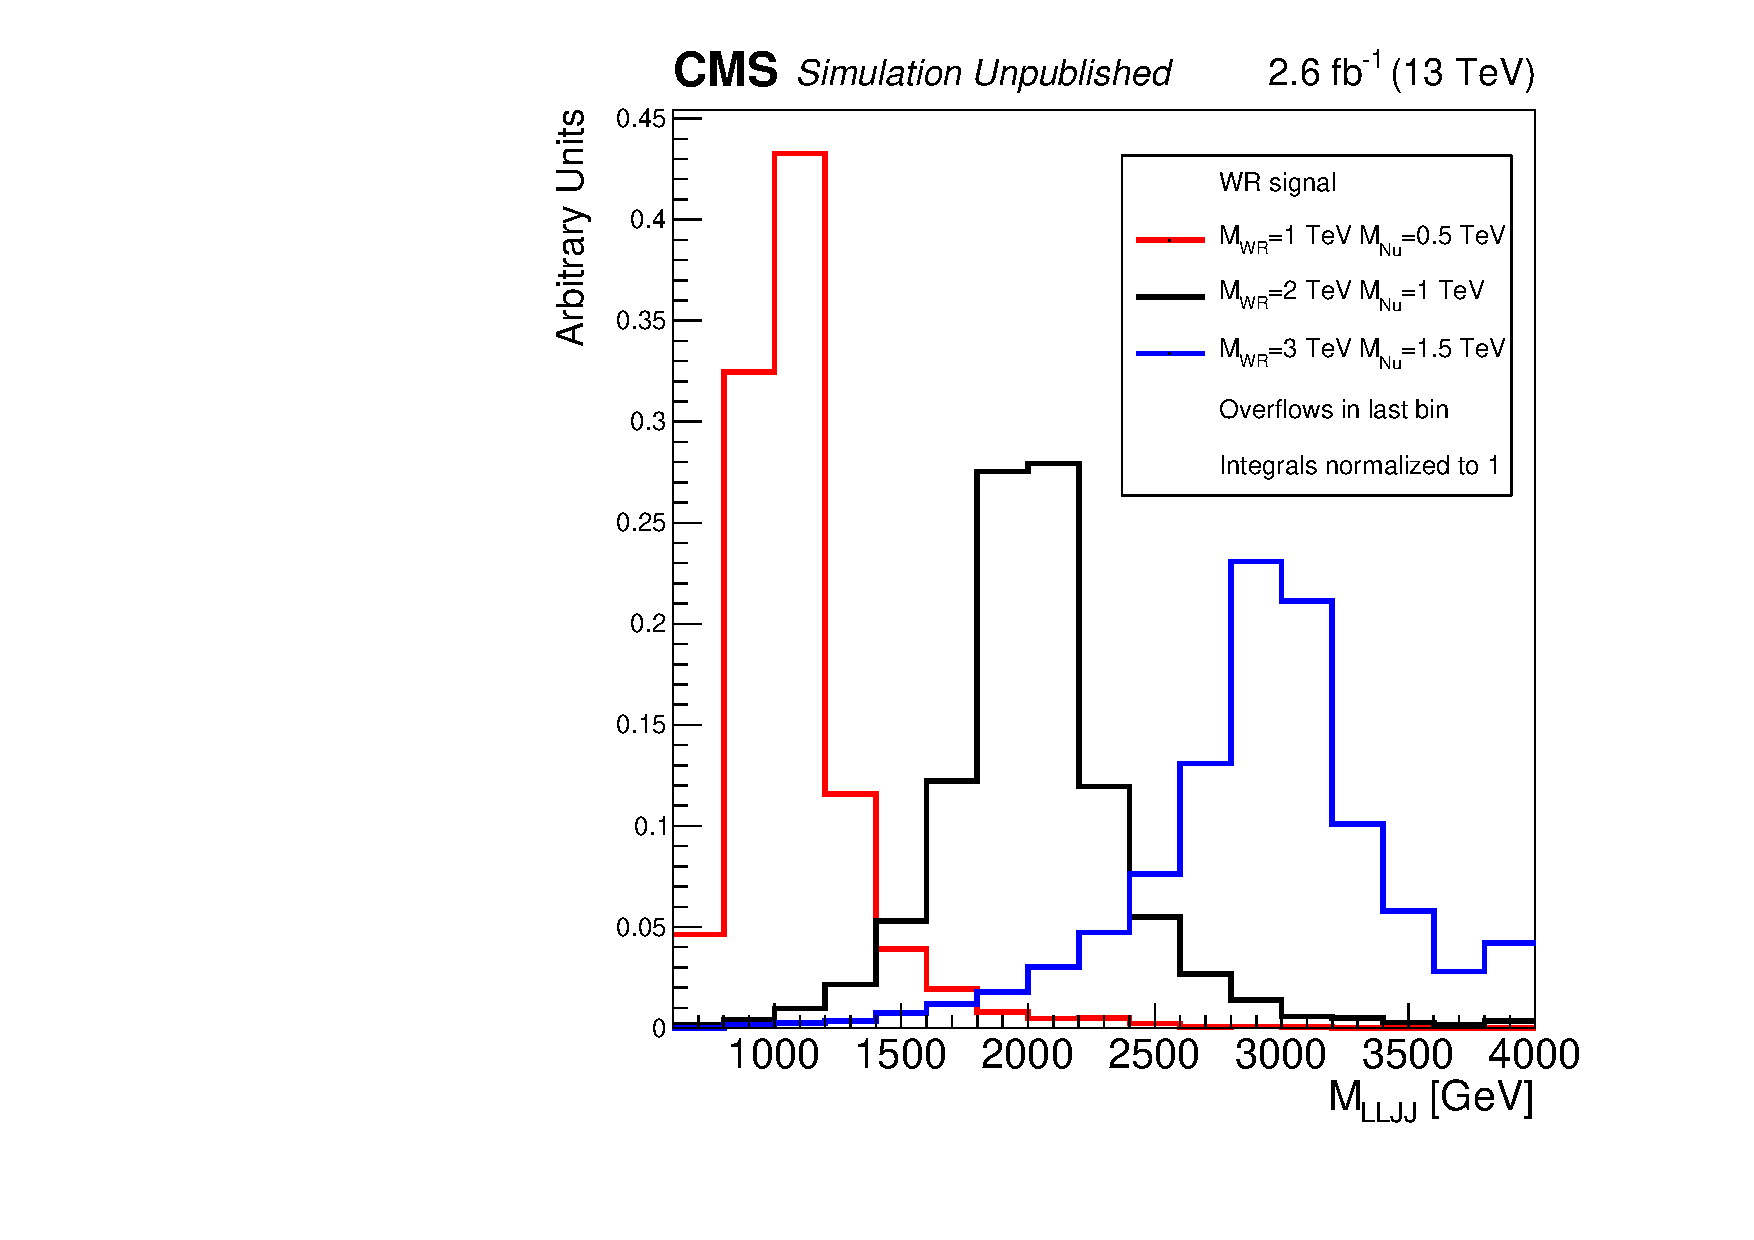
\includegraphics[width=0.45\textwidth]{figures/Mlljj_signalRegionCuts_severalWrSignals_EE.pdf}
	}
	\subfigure{
		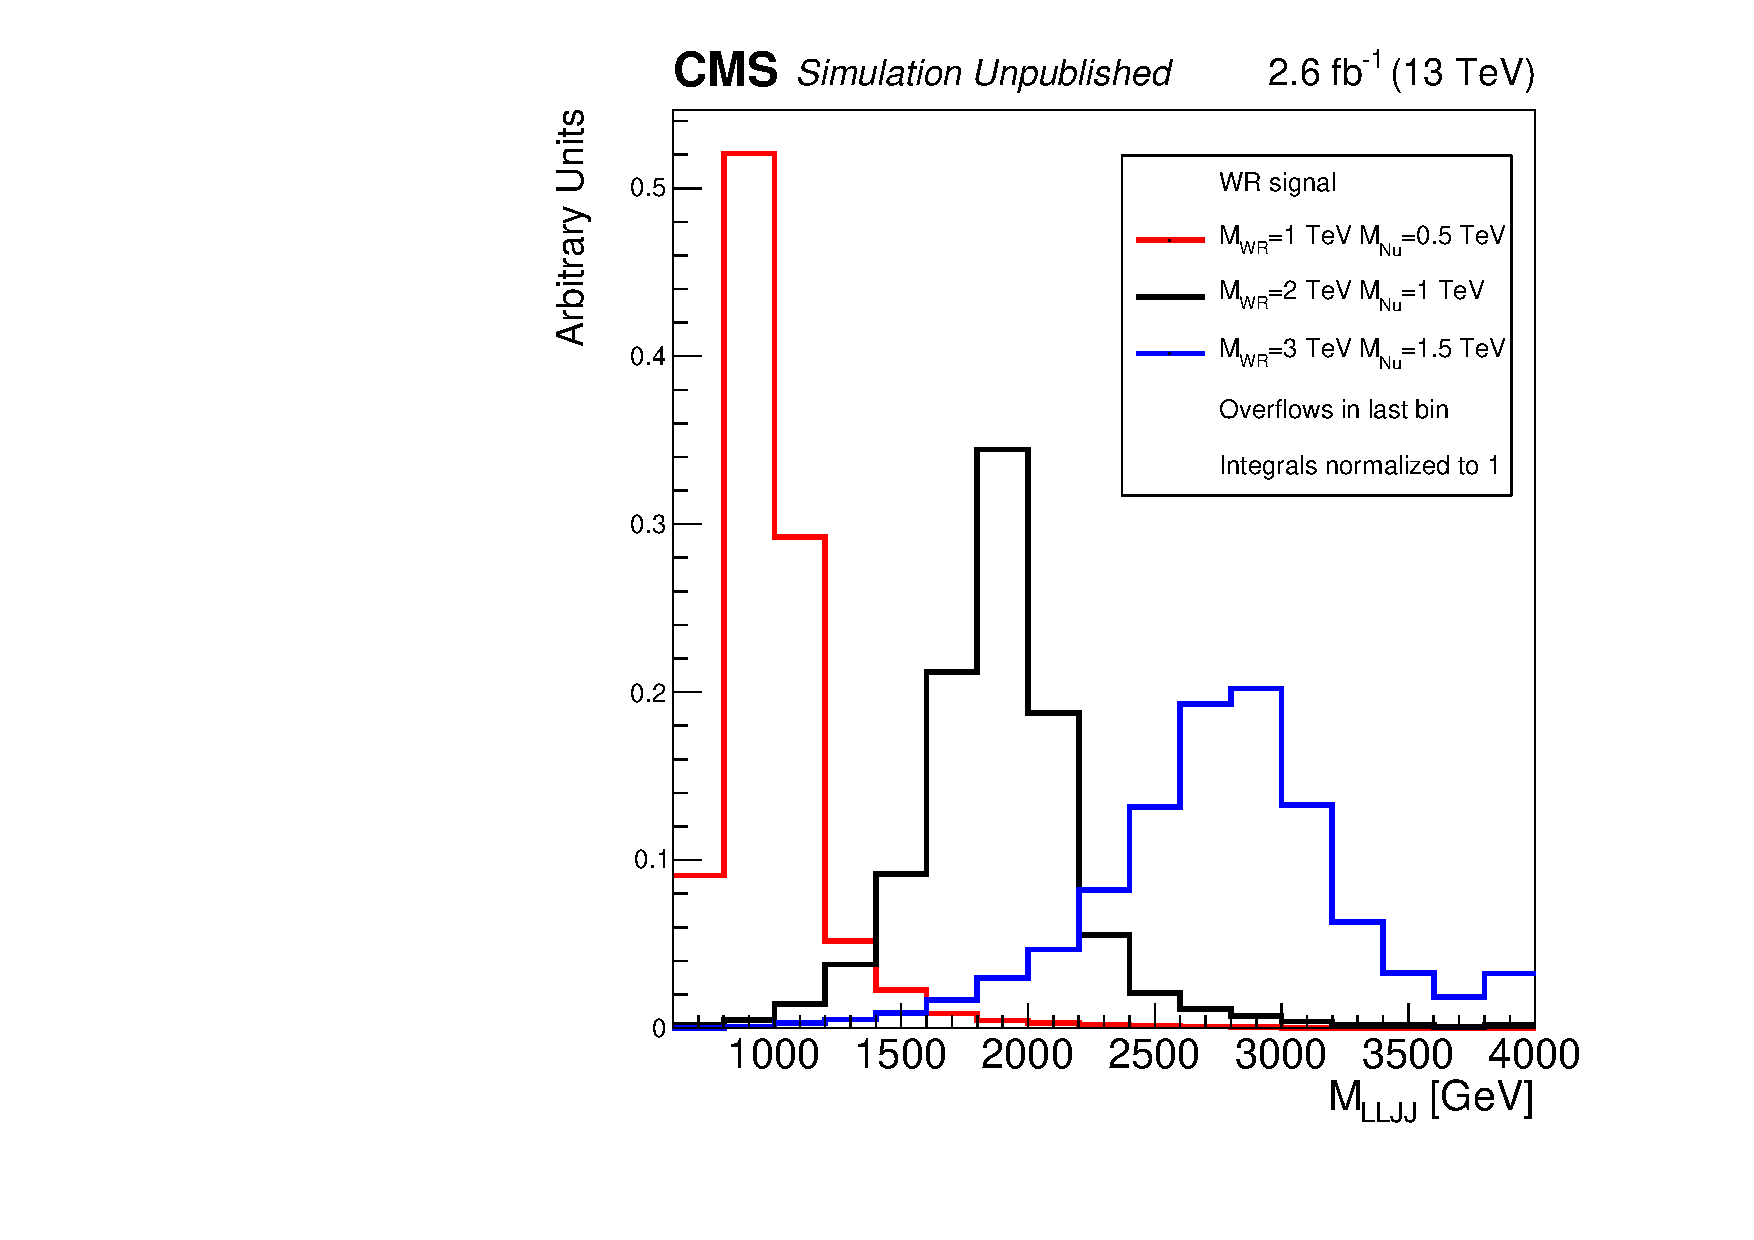
\includegraphics[width=0.45\textwidth]{figures/Mlljj_signalRegionCuts_severalWrSignals_MuMu.pdf}
	}
	\label{fig:signalShapesAfterSelection}
	\caption{$\Mlljj$ distribution after all selections for several \WR signal hypotheses in the $ee$ (left) and $\mu\mu$ (right) 
		channels.  The tails of the distribution grow as \mWR increased.}
\end{figure}

The SM backgrounds that passed the signal region selection were characterized by $\Mlljj$ 
distributions that decreased rapidly with increasing $\Mlljj$, whereas any \WR signal 
after the same selection appeared as an individual peak in the $\Mlljj$ distribution.  
This distinction motivated the division of the entire $\Mlljj > 600\GeV$ range into finite 
width $\Mlljj$ windows linked to specific \mWR hypotheses.  The optimal window size for each 
\mWR hypothesis was determined using the following procedure:

\begin{itemize}
	\item $\sim$150 $\Mlljj$ windows of different sizes were defined based on the expected width of the \WR $\Mlljj$ distribution.
	\item In each window:
	\begin{itemize}
		\item The number of expected signal events $A$ and all SM background events $B$ were calculated.
		\item A Poisson distribution was made with mean equal to $B$, and a random number $C$ representing 
			the number of measured events in the window was pulled from the Poisson distribution.
		\item Using the procedure described in Chapter \ref{sec:searchResults}, the probability that $C$ 
			was measured due to a fluctuation in $A$ and $B$ was calculated, and was rescaled into an 
			upper limit on the \WR cross section.  The size of fluctuations of $A$ and $B$ only depended 
			on their statistical uncertainties.
		\item The cross section limit calculation was repeated 300 times, and each time a new random 
			number $C$ was pulled from the Poisson distribution with mean $B$.  The median value of 
			all 300 limits was taken as the cross section upper limit for the window.
	\end{itemize}
	\item The window that minimized the \WR cross section upper limit was used with the \mWR hypothesis.
\end{itemize}

The $\Mlljj$ window optimization yielded the windows listed in Table \ref{tab:masscuts}.  The windows 
overlapped in $\Mlljj$ because one event with a unique $\Mlljj$ value was compatible with several 
\mWR hypotheses.  In each window the number of events observed in data, and expected from \WR 
signal and all SM backgrounds were counted.  In calculating the expected \WR signal events, only 
the \mWR hypothesis used to optimize the window was considered.  The effect of uncertainties on 
expected event estimates were calculated in each window using procedures described in the next 
section.

\begin{table}[h]
\caption{$\Mlljj$ window ranges that minimized the expected upper limit on the \WR cross section at different \mWR values.}
\label{tab:masscuts}
\centering
\begin{tabular}{|c|r@{ - }l|r@{ - }l|} \hline
\mWR (\GeV) & \multicolumn{4}{c|}{\Mlljj window (\GeV)}  \\\hline
& \multicolumn{2}{c|}{Electrons}  & \multicolumn{2}{c|}{Muons}  \\  \hline
 800  & 700       &  1100       &  700       &  1200      \\  \hline
1000  & 900       &  1300       &  900       &  1400      \\  \hline
1200  & 1100       &  1550       &  1100       &  1650      \\  \hline
1400  & 1250       &  1750       &  1300       &  1850      \\  \hline
1600  & 1450      &  2000       &  1500      &  2100      \\  \hline
1800  & 1600      &  2250       &  1600      &  2300      \\  \hline
2000  & 1850      &  2550       &  1850      &  2600      \\  \hline
2200  & 2000      &  2800       &  2000      &  2850      \\  \hline
2400  & 2150      &  3100       &  2150      &  3100      \\  \hline
2600  & 2250      &  3400       &  2300      &  3400      \\  \hline
2800  & 2350      &  3700       &  2400      &  3700      \\  \hline
3000  & 2500      &  4000       &  2500      &  3950      \\  \hline
3200  & 2550      &  4300       &  2700      &  4250      \\  \hline
3600  & 2700      &  4900       &  2900      &  4850      \\  \hline
3800  & 2750      &  5200       &  2950      &  5150      \\  \hline
4000  & 2800      &  5500       &  3000      &  5450      \\  \hline
4200  & 2800      &  5750       &  3100      &  5750      \\  \hline
4400  & 2850      &  6050       &  3150      &  6100      \\  \hline
4600  & 2850      &  6300       &  3150      &  6400      \\  \hline
4800  & 2850      &  6600       &  3200      &  6700      \\  \hline
5000  & 2900      &  6850       &  3200      &  7000      \\  \hline
5200  & 2900      &  7050       &  3200      &  7300      \\  \hline
5600  & 2900      &  7500       &  3200      &  7850      \\  \hline
5800  & 2950      &  7700       &  3200      &  8150      \\  \hline
6000  & 2950      &  7900       &  3200      &  8400      \\  \hline
\end{tabular}
\end{table}


%%%%%%%%%%%%%%%%%%%%%%%%%%%%%%%%%%%%%%%%%%%%%%%%%%%%%%%%%%%%%%%%%%%%%%%%%%%%%%%%
% Uncertainties 
%%%%%%%%%%%%%%%%%%%%%%%%%%%%%%%%%%%%%%%%%%%%%%%%%%%%%%%%%%%%%%%%%%%%%%%%%%%%%%%%
\section{Uncertainties}
\label{sec:uncertainties}
%%%%%%%%%%%%%%%%%%%%%%%%%%%%%%%%%%%%%%%%%%%%%%%%%%%%%%%%%%%%%%%%%%%%%%%%%%%%%%%%
In each window the estimated number of expected signal and background events were subject to 
many sources of uncertainty.  The magnitude of each uncertainty was estimated using a technique 
approved by the CMS Collaboration, and the effect of each on the search results was quantified 
as percentage uncertainties on the expected number of events in each $\Mlljj$ window.

\subsection{Dominant Uncertainties}
\label{sec:dominantUncs}

\subsubsection{Energy and Lepton Identification Uncertainties}
\label{sec:enrgyLeptIdUncs}
The impacts of lepton and jet energy uncertainties, and simulated lepton ID uncertainties on 
expected signal and background events was estimated simultaneously, but ignoring other 
uncertainties.  In a set of data or simulated events, some of which passed the full selection, 
varying the measured energies of leptons and jets by their uncertainties resulted in the following:

\begin{itemize}
	\item Events that failed the full selection without any uncertainty variations suddenly passed the 
		selection after varying the energies.
	\item Events that passed the full selection without any uncertainty variations suddenly failed the 
		selection after varying the energies.
	\item Events that passed the full selection without any uncertainty variations again passed the 
		selection after varying the energies, but different leptons or jets were selected, and 
		as a result the events migrated to other $\Mlljj$ windows.
	\item Events that passed the full selection without any uncertainty variations again passed the 
		selection after varying the energies, the same leptons and jets were selected as if no 
		variations were applied, and the events fell in the same $\Mlljj$ windows.
	\item Events that passed the full selection without any uncertainty variations again passed the 
		selection after varying the energies, the same leptons and jets were selected as if no 
		variations were applied, but the variations moved the events to other $\Mlljj$ windows.
\end{itemize}

Only the effect of lepton and jet energy uncertainties could cause an event to suddenly pass or fail 
the selection when, without these uncertainties, the opposite occurred, or cause an event to pass the 
selection but migrate to other $\Mlljj$ windows.  The effect of lepton ID uncertainties, which 
only affected simulated events, was estimated at the same time simply for convenience, and had no 
effect on the $\Mlljj$ value of an event that passed the selection.

The magnitudes of lepton and jet energy and ID uncertainties varied with lepton and jet kinematic variables, 
including energy and $(\eta,\phi)$ trajectory, and were estimated and validated independent of all physics 
analyses.  These uncertainties and a brief description of them are listed in Table \ref{tab:energyAndIdUncertainties}.

\begin{table}[ht]
	\caption{Brief descriptions of all uncertainties that affected the $\Mlljj$ value of events with at 
	least two charged leptons and two jets.  All uncertainties affected events in data and simulations, 
except lepton ID uncertainties.}
  \label{tab:energyAndIdUncertainties}
  \centering
    \begin{tabular}{c|c}
		Uncertainty & Description                               \\
      \hline
	  jet energy scale & Uncertainty on the fixed energy scale used to calibrate the energy of jets. \\
 jet energy resolution & Uncertainty on the resolution with which jet energies were measured. \\
   lepton energy scale & Analogous to the jet energy scale uncertainty, but for charged leptons. \\
 lepton energy resolution & Analogous to the jet energy resolution uncertainty, but for charged leptons. \\
lepton ID & Uncertainty on lepton ID weights applied to simulated events, see Chapters \ref{sec:muonRecoAndSelection,sec:electronRecoAndSelection}. \\
  \hline
  \end{tabular}
\end{table}

The impact of these uncertainties on estimates of expected background and signal events was 
determined by applying the following procedure\footnote{This procedure was reviewed and approved by the CMS Collaboration.} 
independently to simulated $\DY$ events, simulated $\WR \rightarrow \ell\ell jj$ events, and 
$e\mu$ data events that were used to estimate the top quark background:

\begin{itemize}
	\item In every event selected by a trigger, but before any lepton or jet selections:
	\begin{itemize}
		\item Eight random numbers were pulled from eight different Gaussians, each with mean 0 and variance 1.
		\item Two random numbers multiplied the electron energy scale and resolution uncertainty of each electron, and these 
			energy changes were propagated to every electron.  In simulated events, a third random number multiplied 
			the ID weight uncertainty of each electron, and the change in weight was propagated to the total event weight 
			after all selections.
		\item Three other random numbers were used to determine the effect of muon energy and ID uncertainties (ID uncertainty 
			only considered in simulated events) following the same procedure used for electrons.
		\item The remaining two random numbers multiplied the jet energy scale and resolution uncertainty of each jet, and 
			these energy changes were propagated to every jet.
	\end{itemize}
	\item The offline selections described in Chapter \ref{sec:event_selection_chapter} were applied to each event.  If all 
		requirements were met and a \WR candidate was built, the event was placed in one or more $\Mlljj$ windows based on 
		the $\Mlljj$ of the \WR candidate.
\end{itemize}

This procedure was iterated 3200 times for every event.  For each signal and background process, distributions 
of the number of events in each $\Mlljj$ window for all 3200 iterations were made, of which an example  
is shown in Figure \ref{fig:effectOfEnergyIdUncerts}.  For each process in an $\Mlljj$ window, the 
distribution's standard deviation represented the uncertainty in the expected number of events due 
to energy and ID uncertainties.  A summary of the expected event uncertainties due to energy and ID 
uncertainties in one $\Mlljj$ window is shown in Table \ref{tab:impactOfEnergyIdUncerts}.

\begin{figure}[h]
	\centering
	
\includegraphics[width=1.0\textwidth]{figures/missingImage.png}
	\caption{The number of expected $\WR \rightarrow \mu\mu jj$ signal events with $\mWR = 2.2\TeV$ in the 2.2$\TeV$ 
	$\Mlljj$ window after 3200 iterations of energy and ID uncertainty variations.}
	\label{fig:effectOfEnergyIdUncerts}
\end{figure}

\begin{table}[ht]
	\caption{Impact of energy and ID uncertainties on expected signal and background event counts in the $\Mlljj$ 
		window optimized for the $\mWR = 2.2\TeV$ hypothesis.  All uncertainties are in percentages of expected events.  Unlike the \DY and \WR 
		estimates, the estimate of top quark background in $ee$ and $\mu\mu$ channels is sensitive to electron and muon energy and ID uncertainties.}
  \label{tab:impactOfEnergyIdUncerts}
  \centering
    \begin{tabular}{c|c|c|c}
		Process & Uncertainty sources    & $\Delta($number of $eejj$ events$)$ (\%) & $\Delta($number of $\mu\mu jj$ events$)$ (\%)  \\
      \hline
	  \WR & lepton energy and ID & $1$ & $3$ \\ 
	  \WR & jet energy & $1$ & $1$ \\ 
	  \DY &  lepton energy and ID & $4$ & $7$  \\
	  \DY &  jet energy & $14$ & $11$  \\
	 Top quark background & lepton energy & $8$ & $8$ \\
	 Top quark background & jet energy & $2$ & $2$  \\
  \hline
  \end{tabular}
\end{table}

\subsubsection{Statistical Uncertainty}
\label{sec:statUnc}
The statistical uncertainty in each $\Mlljj$ window was calculated as $\sqrt{\sum w_{i}^{2}}$, where 
$w_{i}$ was the weight of event i, and the sum ran over all events passing the full selection.  As an 
example, consider an $ee$ channel window that has 10 $e\mu$ data events after all selections.  Here 
the estimated top quark background is $0.43 \cdot 10 = 4.3$ events, and the statistical uncertainty is 
$0.43 \cdot \sqrt{10} \sim 1.4$ events, since $e\mu$ data events all have a weight of 1.  However, in 
many $\Mlljj$ windows optimized for $\mWR \geq 3.0\TeV$ hypotheses, zero background events were expected.  
In such windows, the statistical uncertainty was set equal to the average event weight for all selected 
events.  As shown in Table \ref{tab:impactOfStatUncert}, the statistical uncertainty was largest in the 
top quark background estimate.  The statistical uncertainty was the dominant uncertainty in the top 
quark background estimate.

\begin{table}[ht]
	\caption{Impact of statistical uncertainty on the number of expected signal and background events in the $\Mlljj$ 
		window optimized for the $\mWR = 2.2\TeV$ hypothesis.  All uncertainties are in percentages of expected events.}
  \label{tab:impactOfStatUncert}
  \centering
    \begin{tabular}{c|c|c}
		Process & $\Delta($number of $eejj$ events$)$ (\%) & $\Delta($number of $\mu\mu jj$ events$)$ (\%)  \\
      \hline
	  \WR & $1$ & $1$ \\
	  \DY & $6$ & $5$ \\
	 Top quark background & $44$ & $44$  \\
  \hline
  \end{tabular}
\end{table}

\subsubsection{Background Uncertainty from Control Regions}
\label{sec:bkgndNormUnc}
In the control regions discussed in Chapter \ref{sec:backgroundEstimation}, studies of data and 
simulations motivated applying fixed percentage uncertainties to background estimates.  For 
the top quark background estimate, an uncertainty of 10\% on the expected event count, constant 
in $\Mlljj$, was applied.  For the $\DY$ background estimate, an uncertainty of 40\% on the 
expected event count, constant in $\Mlljj$, was applied.  This was the dominant uncertainty in 
the $\DY$ background estimate.

\subsection{Sub-dominant Uncertainties}
\label{sec:subdominantUncs}

\subsubsection{Lepton Reconstruction and Trigger Efficiency Uncertainties}
\label{sec:leptonRecoTriggerEffUnc}
As discussed in Chapters \ref{sec:muonRecoAndSelection,sec:electronRecoAndSelection}, the efficiencies 
of lepton reconstruction and the muon trigger differed between simulated and data events.  These differences 
were corrected by applying $\sim$unity weights to simulated \DY and \WR events based on selected leptons.  
In the $\mu\mu$ channel, the trigger and reconstruction efficiency weights varied with the energy and $\eta$ of selected muons, and the 
number of events in data and simulations available to estimate these efficiency weights determined 
their uncertainties.  The uncertainty on muon reconstruction efficiency weights was negligible.  The muon trigger 
weight for a triggering muon with $\pt < 140\GeV$ had an uncertainty below 0.5\% of the expected event 
count.  For higher $\pt$ muons the trigger weights had much greater uncertainties because fewer data 
events were available: $<$ 3\% uncertainty for triggering muons with $|\eta| < 2.1$, and 5.1\% uncertainty 
for triggering muons with $2.1 < |\eta| < 2.4$.  In the $ee$ channel, one electron reconstruction 
efficiency weight was calculated for all electrons, and the maximum difference between this inclusive 
weight and an $\Et, \eta$ dependent weight was taken as the uncertainty on the weight.  This uncertainty 
was 2\%, and was applied to \DY and \WR estimates in all $\Mlljj$ windows.

\subsubsection{Cross Section, Luminosity, Pileup and PDF Uncertainties}
\label{sec:crossSxnPileupPdfUnc}
As \DY and \WR expected event counts were estimated from simulated events, these estimates were affected 
by additional uncertainties that did not affect the top quark background estimate: uncertainties 
in cross section, luminosity, pileup, and parton distribution functions (PDFs) and QCD scale uncertainties.  By comparing \DY datasets simulated 
with different generators to data, the \DY cross section uncertainty was determined as 2\% (1\%) in the 
$ee$ $\mu\mu$ channel.  \WR datasets simulated with different generators were not available, so the \WR 
cross section uncertainty was determined by uncertainties in SM coupling constants and particle masses 
hard coded into \PYTHIA.  The total effect of these uncertainties decreased as more events were generated, 
and as a result the 50000 event \WR datasets used here had negligible cross section uncertainties.

The number of expected \WR and \DY events was normalized to the measured integrated luminosity of data.  
The integrated luminosity of data was measured with a 2.7\% uncertainty, and this uncertainty translated 
into a 2.7\% uncertainty on the number of expected \WR and \DY events in every $\Mlljj$ window.

Pileup weights $w_{PUi}$ applied to simulated events were derived assuming the pileup distribution in data followed 
a specific shape, which was sensitive to the vertex reconstruction performance of the tracker.  Uncertainties 
and inefficiencies in vertex reconstruction lead to an uncertainty in the pileup 
distribution of data.  The effect of this uncertainty was estimated by shifting the entire pileup distribution 
in data, without changing its shape, higher (lower) to change the mean pileup value in data by +5\% (-5\%).  
New pileup weights $w_{PUj}$ were calculated for the upward and downward shifts, and the pileup uncertainty 
was calculated as the maximum percentage change in events in $\Mlljj$ windows using the original and new 
weights.  For \DY and \WR event estimates, the pileup uncertainty was 3\% or less in all $\Mlljj$ windows 
and \mWR values.

\DY and \WR events were simulated using:

\begin{itemize}
	\item One parton distribution function (PDF) that described how momenta were distributed amongst quark and 
		gluon constituents of colliding protons.  \WR simulations used NNPDF23 \cite{nnpdf23}, \DY simulations 
		used NNPDF30 \cite{nnpdf30}, and both PDFs were characterized by fixed value coefficients with uncertainties.
	\item One renormalization scale value $\mu_{R}$ (in $\GeV$) that determined the QCD coupling strength $\alpha_{QCD}$.
	\item One factorization scale value $\mu_{F}$ (in $\GeV$), which allowed QCD interactions with low momentum transfer 
		$k_{low} \ll \mu_{F}$ to be simulated independently of QCD interactions with high momentum transfer 
		$k_{high} \sim \mu_{F}$ (see \cite{qcdFactorizationTheory} for more details).
\end{itemize}

The effect of uncertainties in the PDF, $\mu_{R}$ and $\mu_{F}$ values were estimated by resimulating \DY and 
\WR events with different PDF coefficients and QCD scale values, and subsequently reapplying all event selections and 
corrections.  To be conservative, the QCD scales were independently increased or decreased by a factor of 2 
(both were doubled, one was not changed while the other was halved, etc), and the maximum percentage change 
in events in an $\Mlljj$ window was used as the QCD scale uncertainty.  The QCD scale uncertainty was added 
in quadrature with the PDF uncertainty for each $\Mlljj$ window.  For \DY events the combined PDF and QCD 
scale uncertainty never exceeded 4\% in any $\Mlljj$ window.  For each \mWR hypothesis, the PDF and QCD scale 
uncertainty was calculated in the $\Mlljj$ window optimized for the specific \mWR hypothesis.  For all \mWR 
hypotheses the QCD scale uncertainty was no more than a few percent for any \mWR, but the PDF uncertainty 
scaled with \mWR, as shown in Table \ref{tab:wrPdfAndQCDscaleUnc}.  Following CMS guidelines, the \WR PDF 
uncertainty was factored into two pieces: one piece that only depends on relativistic kinematics and masses 
(\mWR and \mnul) and affects the $(\eta, \phi)$ acceptance of \WR decay products, and another piece that depends 
on variable, weakly constrained parameters in LRS models and affects the production rate of \WR bosons.  The acceptance 
uncertainty was $\lesssim$ 1\% for all \mWR hypotheses, and was included in the calculation of results.  The 
production rate uncertainty, constituting the majority of the PDF uncertainty, grew with \mWR, but was not 
included when calculating the results because the uncertainty depended on the specific LRS model being tested.  
By excluding this model dependent uncertainty, the results can be interpreted in the context of many LRS models.

\begin{table}[ht]
	\caption{Uncertainty in the number of predicted \WR signal events due to PDF and QCD scale uncertainties.}
  \label{tab:wrPdfAndQCDscaleUnc}
  \centering
    \begin{tabular}{c|c|c}
		\mWR (GeV)                     & $\Delta( eejj$ events$)$ (\%) & $\Delta( \mu\mu jj$ events$)$ (\%)  \\
      \hline
	  1000  & $4$ & $4$ \\
	  2200 & $7$ & $7$ \\
	  3000 & $15$ & $15$ \\
	  4000 & $18$ & $19$ \\
	  \hline
  \end{tabular}
\end{table}

\subsection{Cumulative Uncertainty}
\label{sec:cumulativeUnc}
The net effect of all uncertainty sources on the estimated number of SM background and \WR signal events in 
several $\Mlljj$ windows is shown in Table \ref{tab:expectedEventsAndAllUncs}.  All uncertainties excluding 
the statistical uncertainty were labeled as systematic uncertainties, and their magnitudes were all summed 
in quadrature.  The dominant \DY background uncertainty was the 40\% uncertainty assigned based on disagreement 
between data and simulated events in a control region where good agreement was expected.  The dominant top 
quark background uncertainty was statistical uncertainty, as fewer than 500 $e\mu$ data events passed the 
full selection with $\Mlljj > 600\GeV$.

\begin{table}[htp]
	\caption{For \mWR hypotheses with $M_{\nul} = \frac{1}{2} \mWR$, these are the number of expected \WR signal and background events in each $\Mlljj$ window, and 
	their statistical and systematic uncertainties.  Each uncertainty is listed as a number of events relative to the expected number of events. BG = Backgrounds, DY = \DY }
	\label{tab:expectedEventsAndAllUncs}
	\centering
	\resizebox{1\textwidth}{3.1cm}{\begin{tabular}{|c|c|c|c|c|}
		& \multicolumn{4}{c|}{Electron channel}  \\
		\mWR ($\GeV$) & Signal (exp $\pm$ stat $\pm$ syst) & DY (exp $\pm$ stat $\pm$ syst) & Top quark (exp $\pm$ stat $\pm$ syst) & $\Sigma$ BG (exp $\pm$ stat $\pm$ syst) \\\hline
		1000 & 1196.0 $\pm$ 15.0 $\pm$ 46.0 & 21.11 $\pm$ 1.64 $\pm$ 8.79 & 40.87 $\pm$ 4.2 $\pm$ 4.76 & 61.99 $\pm$ 4.51 $\pm$ 10.0   \\ \hline
		2200 & 38.0 $\pm$ 0.4 $\pm$ 1.5 & 2.66 $\pm$ 0.15 $\pm$ 1.16 & 2.25 $\pm$ 0.99 $\pm$ 0.3 & 4.92 $\pm$ 1.0 $\pm$ 1.2    \\ \hline
		3000 & 7.3 $\pm$ 0.07 $\pm$ 0.27 & 1.02 $\pm$ 0.09 $\pm$ 0.44 & 0.43 $\pm$ 0.43 $\pm$ 0.05 & 1.45 $\pm$ 0.44 $\pm$ 0.45    \\ \hline
		4000 & 1.0 $\pm$ 0.01 $\pm$ 0.04 & 0.65 $\pm$ 0.08 $\pm$ 0.29 & 0.0 $\pm$ 0.43 $\pm$ 0.0 & 0.65 $\pm$ 0.44 $\pm$ 0.29    \\ \hline
	   & \multicolumn{4}{c|}{Muon channel}  \\
		\mWR ($\GeV$) & Signal (exp $\pm$ stat $\pm$ syst) & DY (exp $\pm$ stat $\pm$ syst) & Top quark (exp $\pm$ stat $\pm$ syst) & $\Sigma$ BG (exp $\pm$ stat $\pm$ syst) \\\hline
		1000 & 1805.0 $\pm$ 17.9 $\pm$ 83.1 & 42.16 $\pm$ 2.28 $\pm$ 17.85 & 70.51 $\pm$ 6.82 $\pm$ 7.97 & 112.67 $\pm$ 7.19 $\pm$ 19.55   \\ \hline
		2200 & 52.0 $\pm$ 0.5 $\pm$ 2.5 & 4.97 $\pm$ 0.25 $\pm$ 2.14 & 3.44 $\pm$ 1.51 $\pm$ 0.45 & 8.41 $\pm$ 1.53 $\pm$ 2.18    \\ \hline
		3000 & 9.1 $\pm$ 0.08 $\pm$ 0.39 & 2.62 $\pm$ 0.16 $\pm$ 1.13 & 0.66 $\pm$ 0.66 $\pm$ 0.08 & 3.28 $\pm$ 0.68 $\pm$ 1.13    \\ \hline
		4000 & 1.2 $\pm$ 0.01 $\pm$ 0.05 & 1.37 $\pm$ 0.1 $\pm$ 0.63 & 0.0 $\pm$ 0.66 $\pm$ 0.0 & 1.37 $\pm$ 0.67 $\pm$ 0.63    \\ \hline
	\end{tabular}}
\end{table}


%%%%%%%%%%%%%%%%%%%%%%%%%%%%%%%%%%%%%%%%%%%%%%%%%%%%%%%%%%%%%%%%%%%%%%%%%%%%%%%%
% Results
%%%%%%%%%%%%%%%%%%%%%%%%%%%%%%%%%%%%%%%%%%%%%%%%%%%%%%%%%%%%%%%%%%%%%%%%%%%%%%%%
\section{Results}
\label{sec:searchResults}
Evidence of LRS models was searched for by comparing expected signal and background events to observed data 
events after all selections.  The initial comparison between expectations and observations was made using the 
$\Meejj$ and $\Mmumujj$ distributions, with (Table \ref{tab:expAndObsEvtsWithAllUncs}) and without (Figure 
\ref{fig:obsAndExpMlljj}) applying the $\Mlljj$ window cuts described in Section \ref{sec:massWindows}.

\begin{table}[htp]
	\caption{For \mWR hypotheses with $M_{\nul} = \frac{1}{2} \mWR$, these are the number of expected \WR signal and background events in each $\Mlljj$ window, and 
	their statistical and systematic uncertainties.  Each uncertainty is listed as a number of events relative to the expected number of events. BG = Backgrounds, DY = \DY }
	\label{tab:expAndObsEvtsWithAllUncs}
	\centering
	\resizebox{1\textwidth}{9cm}{\begin{tabular}{|c|c|c|c|c|c|}
			& \multicolumn{5}{c|}{Electron channel}  \\
			\mWR ($\GeV$) & Signal (exp $\pm$ stat $\pm$ syst) & DY (exp $\pm$ stat $\pm$ syst) & Top quark (exp $\pm$ stat $\pm$ syst) & $\Sigma$ BG (exp $\pm$ stat $\pm$ syst) & Data \\\hline
			800 & 2690.0 $\pm$ 36.4 $\pm$ 103.4 & 37.95 $\pm$ 2.54 $\pm$ 15.69 & 107.52 $\pm$ 6.81 $\pm$ 11.62 & 145.48 $\pm$ 7.27 $\pm$ 19.52 & 136.0   \\ \hline
			1000 & 1196.0 $\pm$ 15.0 $\pm$ 46.0 & 21.11 $\pm$ 1.64 $\pm$ 8.79 & 40.87 $\pm$ 4.2 $\pm$ 4.76 & 61.99 $\pm$ 4.51 $\pm$ 10.0 & 64.0    \\ \hline
			1200 & 583.0 $\pm$ 7.2 $\pm$ 23.0 & 14.31 $\pm$ 1.3 $\pm$ 5.9 & 24.25 $\pm$ 3.23 $\pm$ 2.58 & 38.56 $\pm$ 3.49 $\pm$ 6.43 & 43.0    \\ \hline
			1400 & 327.0 $\pm$ 3.8 $\pm$ 12.3 & 10.67 $\pm$ 0.99 $\pm$ 4.44 & 16.15 $\pm$ 2.64 $\pm$ 1.79 & 26.82 $\pm$ 2.82 $\pm$ 4.79 & 23.0    \\ \hline
			1600 & 179.0 $\pm$ 2.0 $\pm$ 6.9 & 7.48 $\pm$ 0.7 $\pm$ 3.12 & 5.96 $\pm$ 1.6 $\pm$ 0.75 & 13.44 $\pm$ 1.75 $\pm$ 3.21 & 10.0    \\ \hline
			1800 & 108.0 $\pm$ 1.2 $\pm$ 4.1 & 5.8 $\pm$ 0.6 $\pm$ 2.52 & 3.05 $\pm$ 1.15 $\pm$ 0.42 & 8.85 $\pm$ 1.29 $\pm$ 2.56 & 6.0     \\ \hline
			2000 & 59.0 $\pm$ 0.6 $\pm$ 2.4 & 3.56 $\pm$ 0.2 $\pm$ 1.49 & 2.21 $\pm$ 0.98 $\pm$ 0.32 & 5.77 $\pm$ 1.0 $\pm$ 1.52 & 1.0     \\ \hline
			2200 & 38.0 $\pm$ 0.4 $\pm$ 1.5 & 2.66 $\pm$ 0.15 $\pm$ 1.16 & 2.25 $\pm$ 0.99 $\pm$ 0.3 & 4.92 $\pm$ 1.0 $\pm$ 1.2 & 2.0     \\ \hline
			2400 & 24.6 $\pm$ 0.26 $\pm$ 0.97 & 1.9 $\pm$ 0.13 $\pm$ 0.87 & 2.1 $\pm$ 0.95 $\pm$ 0.26 & 4.0 $\pm$ 0.96 $\pm$ 0.91 & 3.0     \\ \hline
			2600 & 16.3 $\pm$ 0.17 $\pm$ 0.61 & 1.58 $\pm$ 0.14 $\pm$ 0.7 & 1.43 $\pm$ 0.78 $\pm$ 0.29 & 3.01 $\pm$ 0.79 $\pm$ 0.76 & 2.0     \\ \hline
			2800 & 11.2 $\pm$ 0.11 $\pm$ 0.42 & 1.35 $\pm$ 0.13 $\pm$ 0.59 & 0.47 $\pm$ 0.45 $\pm$ 0.13 & 1.82 $\pm$ 0.46 $\pm$ 0.6 & 2.0     \\ \hline
			3000 & 7.3 $\pm$ 0.07 $\pm$ 0.27 & 1.02 $\pm$ 0.09 $\pm$ 0.44 & 0.43 $\pm$ 0.43 $\pm$ 0.05 & 1.45 $\pm$ 0.44 $\pm$ 0.45 & 2.0     \\ \hline
			3200 & 4.8 $\pm$ 0.05 $\pm$ 0.18 & 0.96 $\pm$ 0.09 $\pm$ 0.42 & 0.34 $\pm$ 0.34 $\pm$ 0.18 & 1.3 $\pm$ 0.35 $\pm$ 0.46 & 2.0     \\ \hline
			3600 & 2.1 $\pm$ 0.02 $\pm$ 0.08 & 0.76 $\pm$ 0.09 $\pm$ 0.35 & 0.0 $\pm$ 0.43 $\pm$ 0.0 & 0.76 $\pm$ 0.44 $\pm$ 0.35 & 1.0     \\ \hline
			3800 & 1.5 $\pm$ 0.01 $\pm$ 0.05 & 0.71 $\pm$ 0.09 $\pm$ 0.32 & 0.0 $\pm$ 0.43 $\pm$ 0.0 & 0.71 $\pm$ 0.44 $\pm$ 0.32 & 1.0     \\ \hline
			4000 & 1.0 $\pm$ 0.01 $\pm$ 0.04 & 0.65 $\pm$ 0.08 $\pm$ 0.29 & 0.0 $\pm$ 0.43 $\pm$ 0.0 & 0.65 $\pm$ 0.44 $\pm$ 0.29 & 1.0     \\ \hline
			4200 & 0.7 $\pm$ 0.01 $\pm$ 0.02 & 0.66 $\pm$ 0.08 $\pm$ 0.3 & 0.0 $\pm$ 0.43 $\pm$ 0.0 & 0.66 $\pm$ 0.44 $\pm$ 0.3 & 1.0     \\ \hline
			4400 & 0.44 $\pm$ 0.0042 $\pm$ 0.0163 & 0.61 $\pm$ 0.08 $\pm$ 0.27 & 0.0 $\pm$ 0.43 $\pm$ 0.0 & 0.61 $\pm$ 0.44 $\pm$ 0.27 & 1.0     \\ \hline
			4600 & 0.29 $\pm$ 0.0028 $\pm$ 0.0109 & 0.61 $\pm$ 0.08 $\pm$ 0.28 & 0.0 $\pm$ 0.43 $\pm$ 0.0 & 0.61 $\pm$ 0.44 $\pm$ 0.28 & 1.0     \\ \hline
			4800 & 0.2 $\pm$ 0.0019 $\pm$ 0.0074 & 0.61 $\pm$ 0.08 $\pm$ 0.28 & 0.0 $\pm$ 0.43 $\pm$ 0.0 & 0.61 $\pm$ 0.44 $\pm$ 0.28 & 1.0     \\ \hline
			5000 & 0.14 $\pm$ 0.0013 $\pm$ 0.005 & 0.56 $\pm$ 0.08 $\pm$ 0.26 & 0.0 $\pm$ 0.43 $\pm$ 0.0 & 0.56 $\pm$ 0.44 $\pm$ 0.26 & 1.0     \\ \hline
			5200 & 0.09 $\pm$ 0.0008 $\pm$ 0.0033 & 0.56 $\pm$ 0.08 $\pm$ 0.26 & 0.0 $\pm$ 0.43 $\pm$ 0.0 & 0.56 $\pm$ 0.44 $\pm$ 0.26 & 1.0     \\ \hline
			5600 & 0.04 $\pm$ 0.0004 $\pm$ 0.0015 & 0.56 $\pm$ 0.08 $\pm$ 0.26 & 0.0 $\pm$ 0.43 $\pm$ 0.0 & 0.56 $\pm$ 0.44 $\pm$ 0.26 & 1.0     \\ \hline
			5800 & 0.03 $\pm$ 0.0002 $\pm$ 0.001 & 0.51 $\pm$ 0.08 $\pm$ 0.23 & 0.0 $\pm$ 0.43 $\pm$ 0.0 & 0.51 $\pm$ 0.44 $\pm$ 0.23 & 1.0     \\ \hline
			6000 & 0.02 $\pm$ 0.0002 $\pm$ 0.0007 & 0.51 $\pm$ 0.08 $\pm$ 0.23 & 0.0 $\pm$ 0.43 $\pm$ 0.0 & 0.51 $\pm$ 0.44 $\pm$ 0.23 & 1.0     \\ \hline
		& \multicolumn{5}{c|}{Muon channel}  \\
			\mWR ($\GeV$) & Signal (exp $\pm$ stat $\pm$ syst) & DY (exp $\pm$ stat $\pm$ syst) & Top quark (exp $\pm$ stat $\pm$ syst) & $\Sigma$ BG (exp $\pm$ stat $\pm$ syst) & Data \\\hline
			800 & 3966.0 $\pm$ 44.4 $\pm$ 176.2 & 73.29 $\pm$ 6.11 $\pm$ 30.45 & 174.32 $\pm$ 10.72 $\pm$ 18.79 & 247.61 $\pm$ 12.34 $\pm$ 35.78 & 244.0   \\ \hline
			1000 & 1805.0 $\pm$ 17.9 $\pm$ 83.1 & 42.16 $\pm$ 2.28 $\pm$ 17.85 & 70.51 $\pm$ 6.82 $\pm$ 7.97 & 112.67 $\pm$ 7.19 $\pm$ 19.55 & 121.0   \\ \hline
			1200 & 872.0 $\pm$ 8.1 $\pm$ 43.4 & 24.23 $\pm$ 1.74 $\pm$ 10.07 & 38.5 $\pm$ 5.04 $\pm$ 4.07 & 62.73 $\pm$ 5.33 $\pm$ 10.86 & 57.0    \\ \hline
			1400 & 441.0 $\pm$ 4.0 $\pm$ 22.9 & 17.04 $\pm$ 1.42 $\pm$ 7.02 & 18.94 $\pm$ 3.53 $\pm$ 2.06 & 35.98 $\pm$ 3.81 $\pm$ 7.32 & 24.0    \\ \hline
			1600 & 244.0 $\pm$ 2.2 $\pm$ 13.3 & 12.71 $\pm$ 1.01 $\pm$ 5.31 & 6.56 $\pm$ 2.07 $\pm$ 1.08 & 19.27 $\pm$ 2.31 $\pm$ 5.42 & 17.0    \\ \hline
			1800 & 150.0 $\pm$ 1.3 $\pm$ 6.7 & 10.94 $\pm$ 0.41 $\pm$ 4.66 & 5.24 $\pm$ 1.86 $\pm$ 0.68 & 16.18 $\pm$ 1.9 $\pm$ 4.71 & 12.0    \\ \hline
			2000 & 82.0 $\pm$ 0.7 $\pm$ 4.3 & 6.52 $\pm$ 0.29 $\pm$ 2.81 & 3.44 $\pm$ 1.51 $\pm$ 0.45 & 9.96 $\pm$ 1.53 $\pm$ 2.85 & 8.0     \\ \hline
			2200 & 52.0 $\pm$ 0.5 $\pm$ 2.5 & 4.97 $\pm$ 0.25 $\pm$ 2.14 & 3.44 $\pm$ 1.51 $\pm$ 0.45 & 8.41 $\pm$ 1.53 $\pm$ 2.18 & 5.0     \\ \hline
			2400 & 32.5 $\pm$ 0.28 $\pm$ 1.52 & 3.89 $\pm$ 0.21 $\pm$ 1.69 & 3.2 $\pm$ 1.45 $\pm$ 0.4 & 7.1 $\pm$ 1.47 $\pm$ 1.74 & 4.0     \\ \hline
			2600 & 20.9 $\pm$ 0.18 $\pm$ 0.97 & 3.28 $\pm$ 0.17 $\pm$ 1.4 & 1.31 $\pm$ 0.92 $\pm$ 0.27 & 4.59 $\pm$ 0.94 $\pm$ 1.42 & 4.0     \\ \hline
			2800 & 13.8 $\pm$ 0.12 $\pm$ 0.6 & 2.97 $\pm$ 0.17 $\pm$ 1.28 & 0.66 $\pm$ 0.66 $\pm$ 0.18 & 3.63 $\pm$ 0.68 $\pm$ 1.29 & 4.0     \\ \hline
			3000 & 9.1 $\pm$ 0.08 $\pm$ 0.39 & 2.62 $\pm$ 0.16 $\pm$ 1.13 & 0.66 $\pm$ 0.66 $\pm$ 0.08 & 3.28 $\pm$ 0.68 $\pm$ 1.13 & 4.0     \\ \hline
			3200 & 5.9 $\pm$ 0.05 $\pm$ 0.26 & 1.99 $\pm$ 0.13 $\pm$ 0.9 & 0.0 $\pm$ 0.66 $\pm$ 0.0 & 1.99 $\pm$ 0.67 $\pm$ 0.9 & 1.0     \\ \hline
			3600 & 2.6 $\pm$ 0.02 $\pm$ 0.11 & 1.52 $\pm$ 0.12 $\pm$ 0.69 & 0.0 $\pm$ 0.66 $\pm$ 0.0 & 1.52 $\pm$ 0.67 $\pm$ 0.69 & 1.0     \\ \hline
			3800 & 1.8 $\pm$ 0.02 $\pm$ 0.07 & 1.46 $\pm$ 0.12 $\pm$ 0.66 & 0.0 $\pm$ 0.66 $\pm$ 0.0 & 1.46 $\pm$ 0.67 $\pm$ 0.66 & 1.0     \\ \hline
			4000 & 1.2 $\pm$ 0.01 $\pm$ 0.05 & 1.37 $\pm$ 0.1 $\pm$ 0.63 & 0.0 $\pm$ 0.66 $\pm$ 0.0 & 1.37 $\pm$ 0.67 $\pm$ 0.63 & 1.0     \\ \hline
			4200 & 0.8 $\pm$ 0.01 $\pm$ 0.03 & 1.21 $\pm$ 0.1 $\pm$ 0.55 & 0.0 $\pm$ 0.66 $\pm$ 0.0 & 1.21 $\pm$ 0.67 $\pm$ 0.55 & 1.0     \\ \hline
			4400 & 0.54 $\pm$ 0.0045 $\pm$ 0.0223 & 1.13 $\pm$ 0.09 $\pm$ 0.52 & 0.0 $\pm$ 0.66 $\pm$ 0.0 & 1.13 $\pm$ 0.67 $\pm$ 0.52 & 1.0     \\ \hline
			4600 & 0.37 $\pm$ 0.003 $\pm$ 0.0151 & 1.14 $\pm$ 0.09 $\pm$ 0.53 & 0.0 $\pm$ 0.66 $\pm$ 0.0 & 1.14 $\pm$ 0.67 $\pm$ 0.53 & 1.0     \\ \hline
			4800 & 0.24 $\pm$ 0.002 $\pm$ 0.0101 & 1.06 $\pm$ 0.08 $\pm$ 0.5 & 0.0 $\pm$ 0.66 $\pm$ 0.0 & 1.06 $\pm$ 0.66 $\pm$ 0.5 & 1.0     \\ \hline
			5000 & 0.18 $\pm$ 0.0014 $\pm$ 0.0074 & 1.06 $\pm$ 0.08 $\pm$ 0.5 & 0.0 $\pm$ 0.66 $\pm$ 0.0 & 1.06 $\pm$ 0.66 $\pm$ 0.5 & 1.0     \\ \hline
			5200 & 0.12 $\pm$ 0.0009 $\pm$ 0.0048 & 1.06 $\pm$ 0.08 $\pm$ 0.5 & 0.0 $\pm$ 0.66 $\pm$ 0.0 & 1.06 $\pm$ 0.66 $\pm$ 0.5 & 1.0     \\ \hline
			5600 & 0.05 $\pm$ 0.0004 $\pm$ 0.0022 & 1.06 $\pm$ 0.08 $\pm$ 0.5 & 0.0 $\pm$ 0.66 $\pm$ 0.0 & 1.06 $\pm$ 0.66 $\pm$ 0.5 & 1.0     \\ \hline
			5800 & 0.04 $\pm$ 0.0003 $\pm$ 0.0015 & 1.06 $\pm$ 0.08 $\pm$ 0.5 & 0.0 $\pm$ 0.66 $\pm$ 0.0 & 1.06 $\pm$ 0.66 $\pm$ 0.5 & 1.0     \\ \hline
			6000 & 0.02 $\pm$ 0.0002 $\pm$ 0.001 & 1.06 $\pm$ 0.08 $\pm$ 0.5 & 0.0 $\pm$ 0.66 $\pm$ 0.0 & 1.06 $\pm$ 0.66 $\pm$ 0.5 & 1.0     \\ \hline
	\end{tabular}}
\end{table}

\begin{figure}[btp]
	\centering
	\subfigure{
		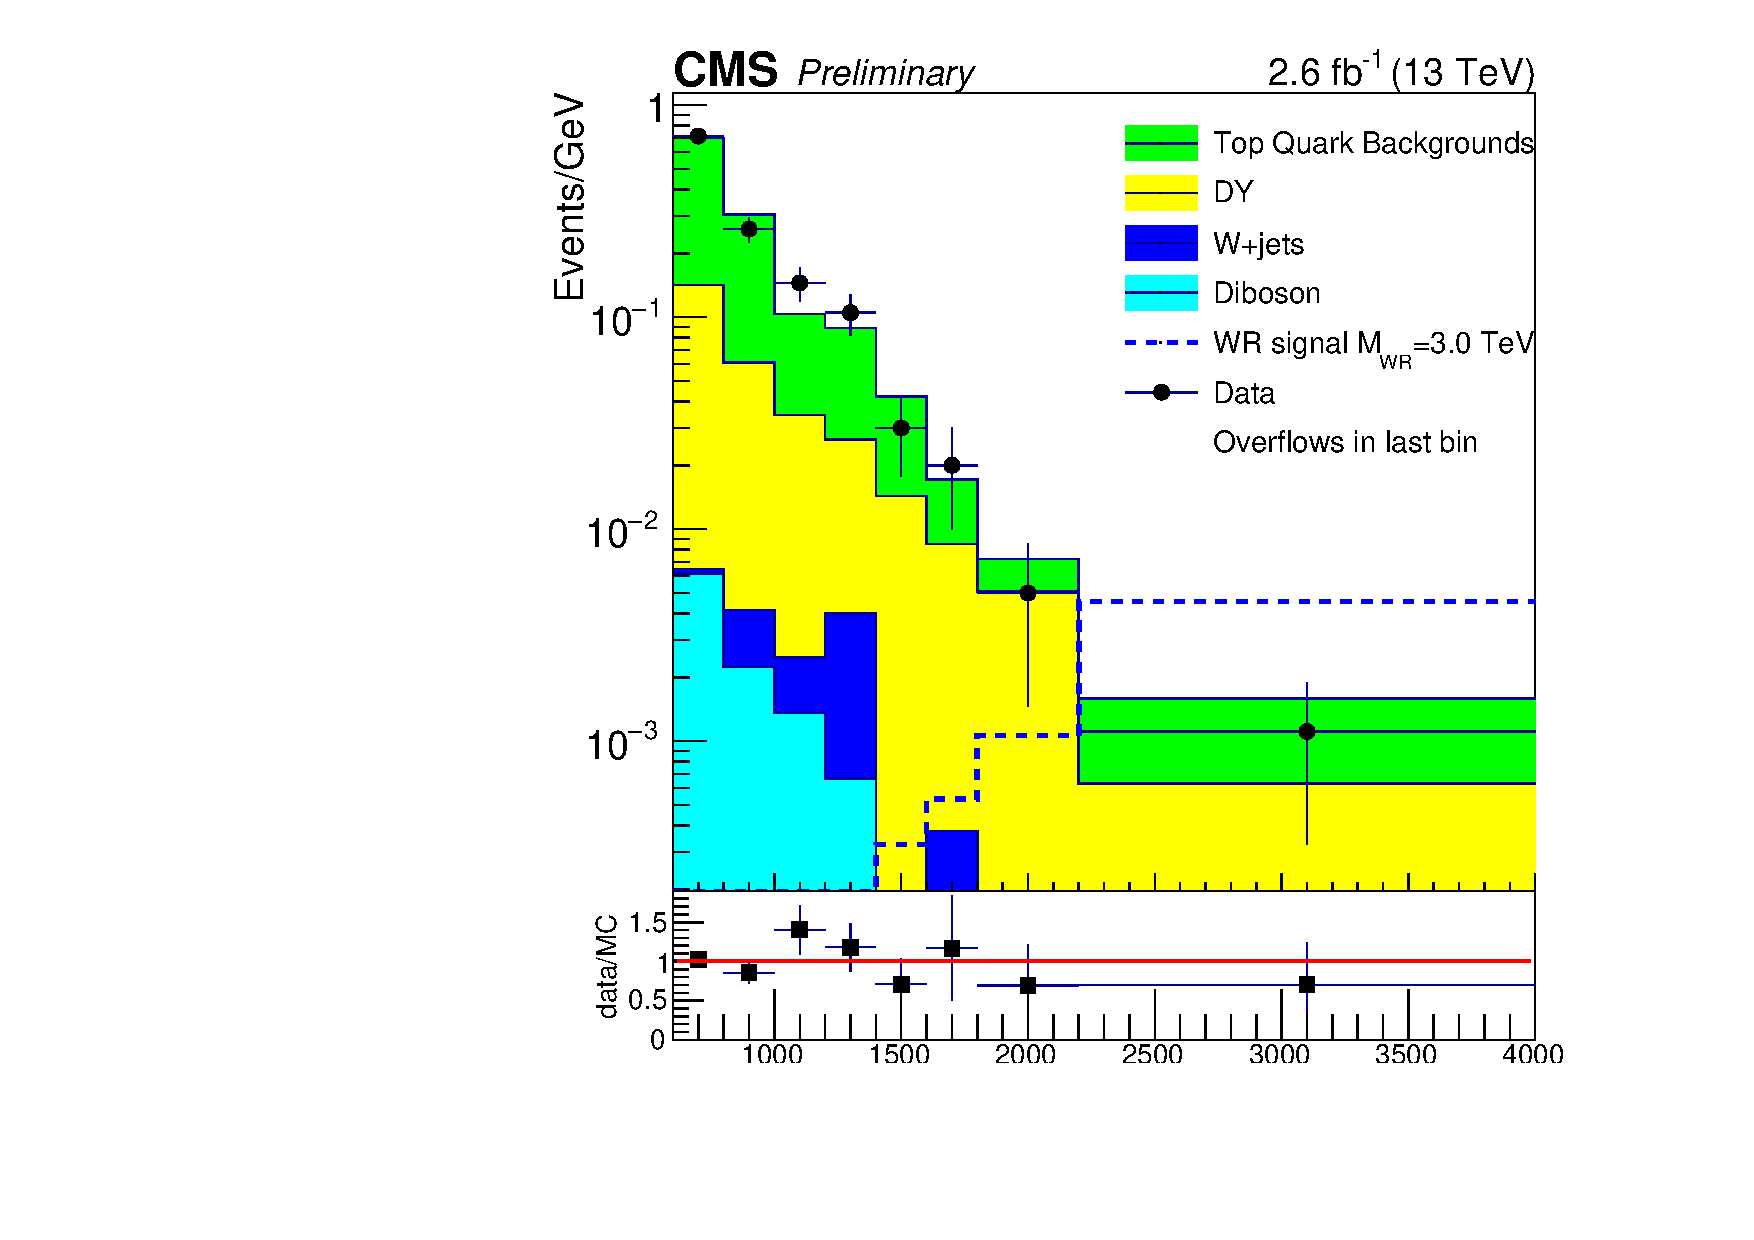
\includegraphics[width=0.45\textwidth]{figures/Mlljj_2012Bins_MWR3000Signal_SignalRegion_EEChannelBkgndMC_DYMadHTAndIncl_TTBarFromData_WithUnblindedData_withRatio_log.pdf}
	}
	\subfigure{
		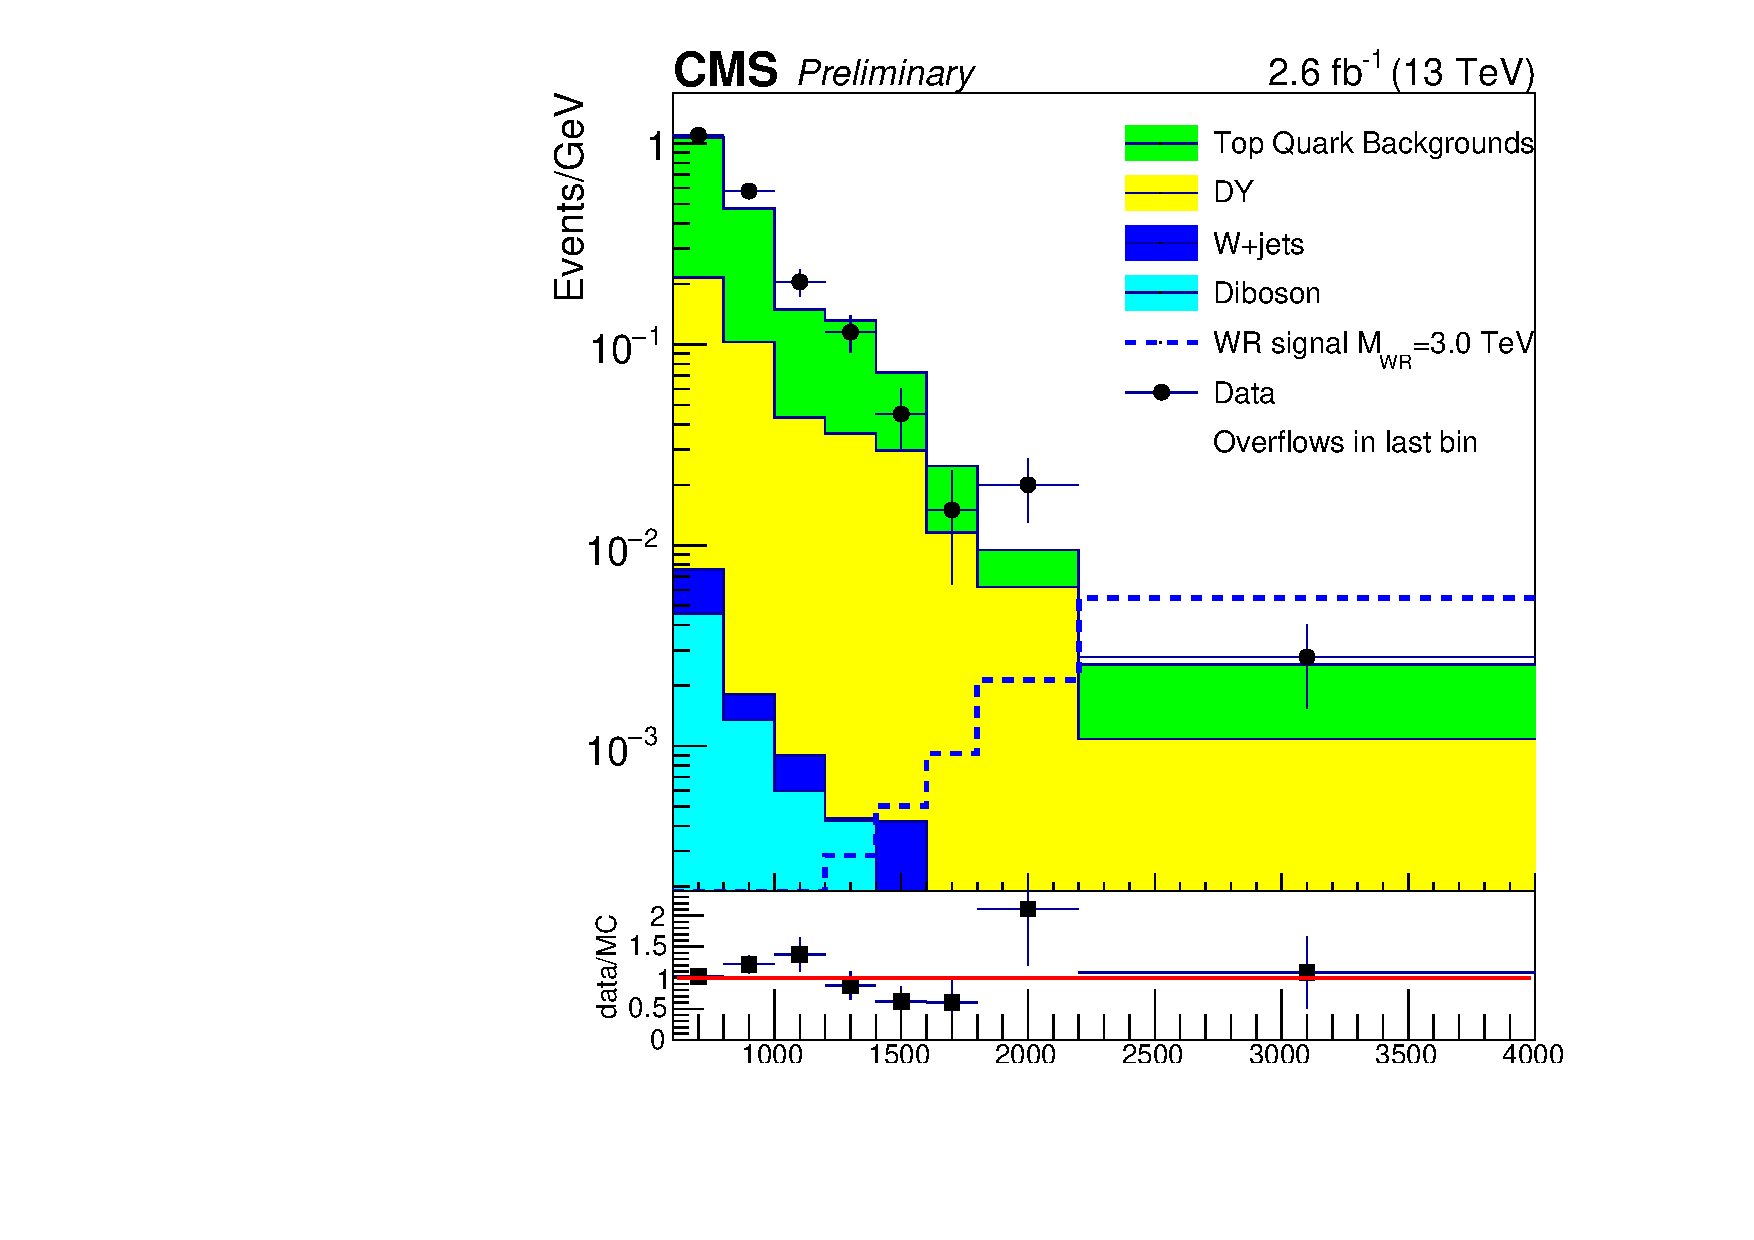
\includegraphics[width=0.45\textwidth]{figures/Mlljj_2012Bins_MWR3000Signal_SignalRegion_MuMuChannelBkgndMC_DYMadHTAndIncl_TTBarFromData_WithUnblindedData_withRatio_log.pdf}
	}
	\label{fig:obsAndExpMlljj}
	\caption{$\Mlljj$ distributions found in data, one simulated \WR signal, and expected backgrounds in the $ee$ ($\mu\mu$) channel on 
		the left (right).}
\end{figure}



%describe how limits are calculated with and without syst uncertainties before showing results
%when explaining limit calculation procedure without syst uncertainties, refer back to 
%Chapter \ref{sec:massWindows}

%%%
%from statistical.tex file of AN
%The probability of the observed number of events being produced by a combination of background and signal with a cross section ($x$) is calculated using the Bayesian approach with the \emph{combine} tool with flat prior. 
%The exclusion limit on the cross section ($x$) is defined as the value for which the posterior likelihood reaches 95\% of the total area under the curve.
%This is repeated for each mass hypothesis.
%
%In order to take into account the uncertainties, pseudo-experiments are performed by the \combine tool varying the expected number of events from signal and background according to the uncertainties as described in the following section. The median of the distribution of the excluded cross section produced by pseudo-experiments and the intervals containing 68\% and 95\% of the pseudo-experiments are then quoted in the ``expected'' limits.
%%%


%%%%%%%%%%%%%%%%%%%%%%%%%%%%%%%%%%%%%%%%%%%%%%%%%%%%%%%%%%%%%%%%%%%%%%%%%%%%%
